\section{Fundamentals of astro-interferometry}
All the development of astro-interferometry is essentially based on one fundamental theorem : the Van Cittert-Zernike theorem. This theorem links the spatial coherence of a far source to its angular brightness distribution. In this section will be explained the limitation of one individual telescope in term of resolution and then introduce the advantages of interferometry. This section is based on \cite{Glindemann} and lectures given by J.P. Berger at Grenoble-INP Phelma. In order to fully understand the concepts lets first introduce the Mutual coherence function.

	\subsubsection{Mutual coherence function}
Lets consider the light field by its optical disturbance function $u(\vec{r},t)$ at position $\vec{r}$ and time $t$. The optical disturbance is proportional to the electrical and magnetic fields of the light.
Lets suppose a far, coherent source illuminating two thin holes situated at position $\vec{r_1}$ and $\vec{r_2}$ (like the young experiment) and forming fringe pattern on a screen. At a point P of the screen and time t, the intensity of the light can be expressed by :
$I(P) = \left< u(P,t)u^*(P,t) \right>$ which can be rewritten if we consider the holes thin enough that the field is constant on their respective surface :
$$
I(P) = \left< \left| u(\vec{r_1},t-\tau_1) \right|^2 \right> + \left< \left| u(\vec{r_2},t-\tau_2) \right|^2 \right> +2\mathcal{R}\left( \left< \left| u(\vec{r_1},t-\tau_1)u^*(\vec{r_2},t-\tau_2) \right| \right> \right)
$$
where $\tau_1$ and $\tau_2$ refers to the travel time of the wave from the pin hole to the point P. The last term of this equation is a term of coherence representing the spatial and spectra properties of the source. From this equation we can generalise the measurement of the coherence of a source by introducing the mutual coherence function (MCF) :
\begin{equation}
\Gamma(\vec{r_1},\vec{r_2}, \tau) = \left< u(\vec{r_1},t+\tau)u^*(\vec{r_2},t)\right> = \lim\limits_{T\rightarrow +\infty}\int_{-T}^T u(\vec{r_1},t+\tau)u^*(\vec{r_2},t)dt
\end{equation} 

In the case of astrointerferometry the two pinholes refers to the telescopes and the source to the observed object. The distance between both telescopes is called the baseline vector $\vec{B}=\vec{r_1}-\vec{r_2}$. 

	\subsubsection{Van Cittert-Zernike theorem}
Now that the MCF has been defined the most fundamental theorem of modern optic can be introduced. We will consider the Van Cittert-Zernike theorem in an adapted to astronomy form. We will consider a surface emitting light. Under the following assumption :
\begin{itemize}
\item[-]The source is incoherent ($\Gamma(P_1,P_2,\tau) = 0 \quad P_1 \neq P_2$ for all $\tau$)
\item[-]The source is small compared to the distance of observation (Fresnel approximation)
\item[-]The source spectral bandwidth is much smaller than its average frequency (quasi-monochromatic approximation).
\end{itemize}

\begin{figure}[htbp!]
\centering
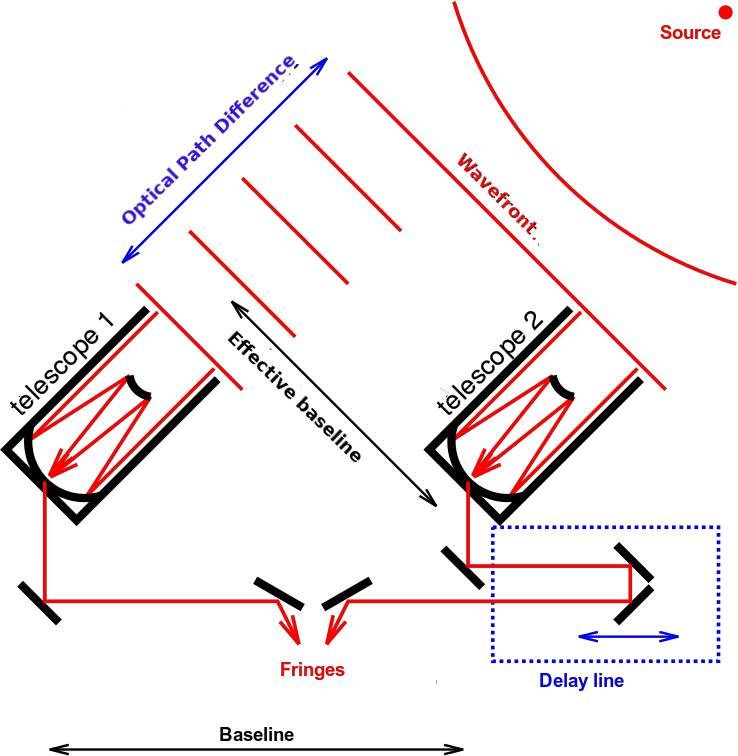
\includegraphics[scale=.3]{../images/scheme.png}
\caption{Scheme of the principle of stellar interferometry. (adaptated from \url{https://fr.wikipedia.org/wiki/Interférométre_optique_à_longue_base})}
\end{figure}

Under those assumptions the Van Cittert-Zernike theorem states that :
$$
\mu(\vec{B}) = \frac{\Gamma(\vec{B},0)}{\sqrt{\Gamma(\vec{r_1},\vec{r_1},0)\Gamma(\vec{r_2},\vec{r_2},0)}} = \frac{\int I_b(\vec{\alpha}) e^{-ik\vec{B} \cdot \vec{\alpha}}}{d\vec{\alpha}}
$$

where alpha is the angle between the line of sight and a point on the observed source and $\mu$ the normalised MCF at $\tau=0$, called the visibility function. $I_b(\vec{\alpha})$ is the angular brightness distribution of the source. This is the force of this theorem, linking the angular brightness distribution of an object to the shape of its interferometric signal. The source can be seen as an infinity of points each interfering at the telescope recombination point. But due to their different position their interferogram are shifted relatively to each other reducing the global visibility. This is this effect that the Van Cittert-Zernike theorem means. Thus the amplitude of visibility $\left| \mu \right|$ lay between 0 and 1.

This theorem explain the usability of interferometry to astronomical purpose but it doesn't explain it's main advantage : an increased angular resolution. 

\begin{figure}[htbp!]
\centering
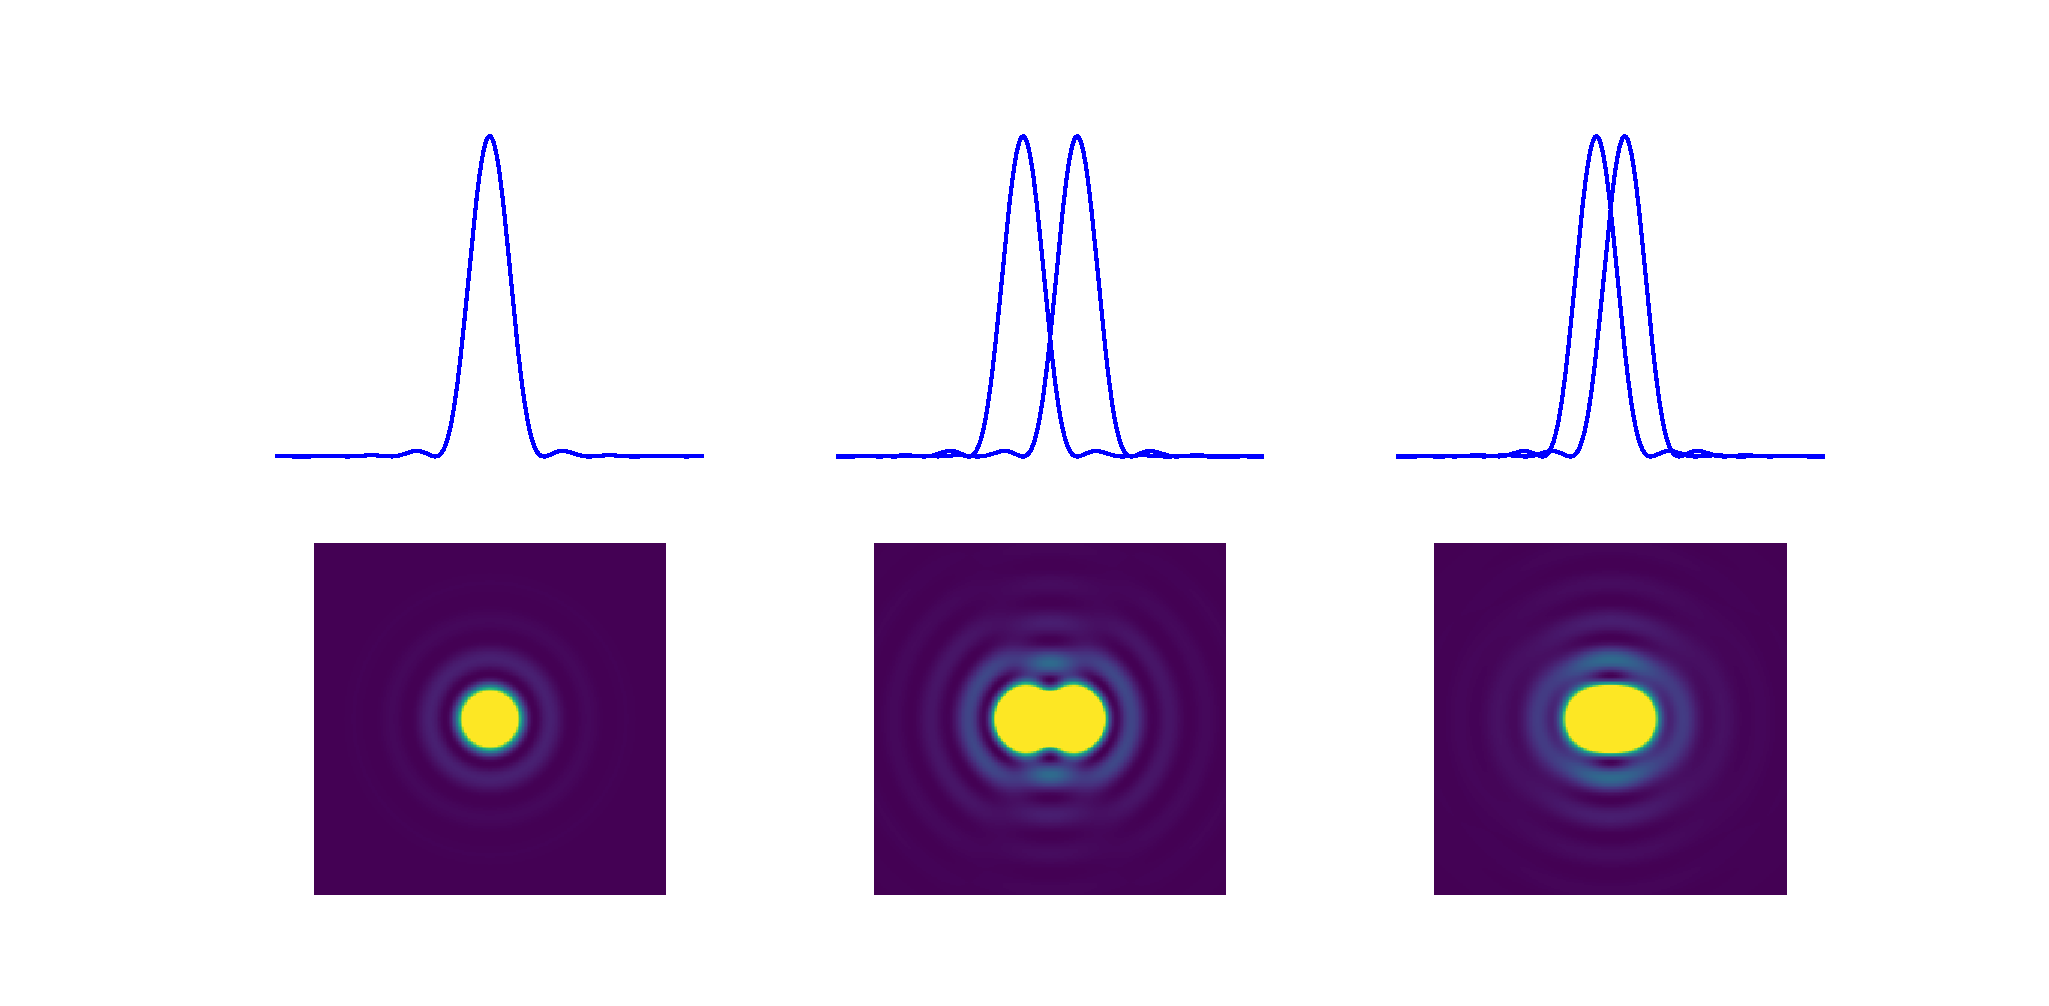
\includegraphics[scale=.3]{../picture/airy.pdf}
\caption{Left : Airy disk / PSF of a circular aperture. Center : Case of the Rayleigh criterion (resolved source). Right : case of an unresolved source}
\label{fig:airy}
\end{figure}

	\subsubsection{Spatial resolution}
Lets now take a simplified example of an individual telescope whose pupil is a disk of diameter D. Fourier's optics tells us that the point spread function (PSF) of such an aperture is a function called Airy's function (see Fig\ref{fig:airy}). 

In the case of 2 source observed, one can define the resolution of the telescope as its capacity to separate two punctual sources. This criterion is called the Rayleigh criterion and is defined as the angular separation such as the first "0" of the image of the first source is at the position of the maximum of the image of the second source. This correspond to an angular resolution of $\Delta \alpha = \frac{1.22\lambda}{D}$. 

One can also define the telescope by its optical transfer function. Doing so it is easy to show that the circular aperture act as a low pass filter (spatial frequency) with a cut off frequency of $f_c = \frac{D}{\lambda}$

When it comes to interferometry with two telescopes separated by a distance $\vec{B}$ (speaking of the effective baseline) observing two stars of same flux separated by a distance $\vec{\rho}$, the visibility function is $\mu(\vec{f})=cos(\pi \vec{f} \dot{} \vec{\rho})$ where $\vec{f}$ if the spatial frequency vector $\vec{f} = \frac{\vec{B}}{\lambda}$ ($\vec{B}$ and $\vec{\rho}$ are vectors defined in the observation plan). In the particular case where $\vec{\rho}= \frac{\lambda}{2\left|\vec{B}\right|} \frac{\vec{B}}{\left|\vec{B}\right|}$ the visibility is equal to zero. Therefore we can deduce that the interferometer formed by two telescopes separated by a distance B is equivalent to an individual telescope of diameter B.  

An interferometer formed by two telescopes separated by a distance B has a resolution of $\frac{\lambda}{2B}$ and gives access to spatial frequency $\frac{B}{\lambda}$. To be able to fit models to measured visibility and to reconstruct an image of the observed object one must do measurements for as many baselines as possible (and also as many wavelength as possible). The purpose of the work presented in this report is to develop a component able to combine at least 4 telescopes (6 different baselines) at the same time making it able to observe fast varying object.


